\documentclass{seminar}
\usepackage{epic,/homes/tiwari/Talks/Special/relative,latexsym,url}
\usepackage{/homes/tiwari/Talks/Special/gastex}
\usepackage{wrapfig}

\usepackage{fancybox}
\usepackage{semlayer}
\usepackage{epsfig}
\usepackage{amssymb}
\usepackage{semcolor}

\graphicspath{{../Powertrain/figures/}{figures/}}

\def\printlandscape{\special{landscape}}    % Works with dvips.
\renewcommand{\printlandscape}{\special{landscape}}
\special{! /landplus90 true store}

\input{/homes/tiwari/Talks/Special/slideprel}
\slideframe{oval}
\usepackage{times} 		%% for PDF purposes

\newcommand\ignore[1]{{{}}}

% \ifpdf\else
%%%%%%%%
% to fix problems making landscape seminar pdfs
% Letter...
%\pdfpagewidth=11truein
%\pdfpageheight=8.5truein
% A4
\pdfpagewidth=297truemm % your milage may vary....
\pdfpageheight=210truemm
\pdfhorigin=1truein     % default value(?), but doesn't work without
\pdfvorigin=1truein     % default value(?), but doesn't work without
%\fi
% -------------------------------------------------------

%---------------------------------------------------------------------
\begin{document}
%---------------------------------------------------------------------
\begin{slide}
\heading{HybridSAL and Relational Abstraction}

\vskip 1.5em
\begin{center}
\begin{tabular}{c}
\underline{\green{Ashish Tiwari}} 
\\
SRI International
\\
Menlo Park
\\
CA 94025
\end{tabular}
\end{center}

\end{slide}
%---------------------------------------------------------------------
\begin{slide}
\heading{Verification Approach}

{\crm{Model check}} {\cem{hybrid}} dynamical systems.

{\cem{Problem:}} How to handle {\cem{differential equations}}?

{\crm{Solution 1}}: Qualitative abstraction
\hspace*{1em}
{\crm{Solution 2}}: Relational abstraction

{\crm{HybridSAL Verification Flow}}:

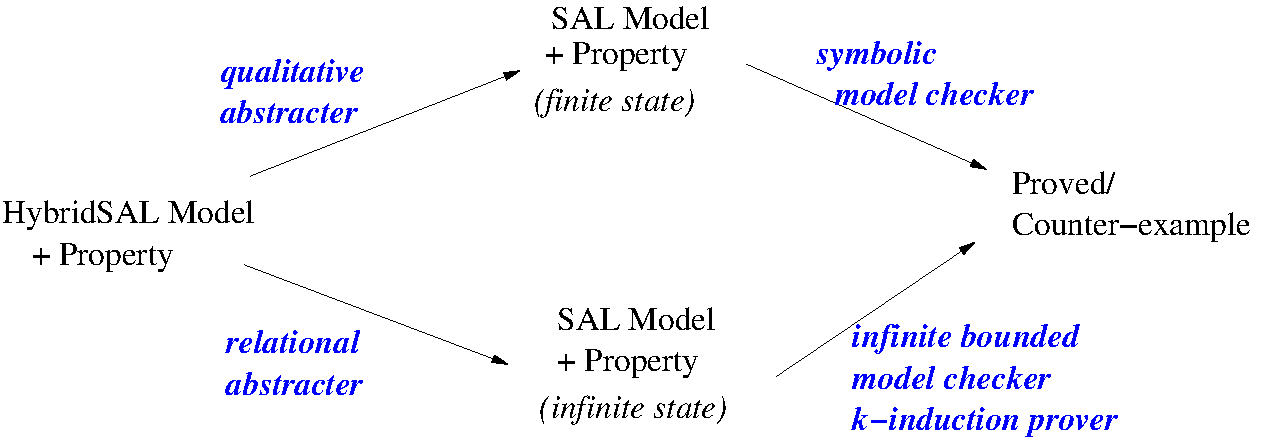
\includegraphics[angle=0,scale=0.5]{hsal-flow}
%\\
%Hybrid Automata + Property
%$\longrightarrow$
%Discrete State Machine + Property
%$\longrightarrow$
%Yes or Counter-example

\end{slide}
% -------------------------------------------------------
\begin{slide}
\heading{Properties}

{\cem{Safety}}: Bad things do not happen

{\crm{Remark:}} Most interesting properties are safety properties

\medskip
Hybrid automaton model is specified in {\cem{HybridSAL}} language
\begin{eqnarray*}
\mathit{{\cem{HybridSAL}}} & = &
 \left\{ \begin{array}{c}
   \mbox{language for state transition systems}, {\cem{SAL}} + 
   \\
   \mbox{syntax for continuous dynamics} \end{array}\right.
\end{eqnarray*}

\medskip
Property is specified in {\cem{linear temporal logic}}
\begin{eqnarray*}
\mathit{{\cem{LTL}}} & = & \mbox{predicate logic} + \mbox{temporal operators}
\end{eqnarray*}

\end{slide}
% -------------------------------------------------------
\begin{slide}
\heading{Hybrid Verification: Motivating Example}

\begin{center}
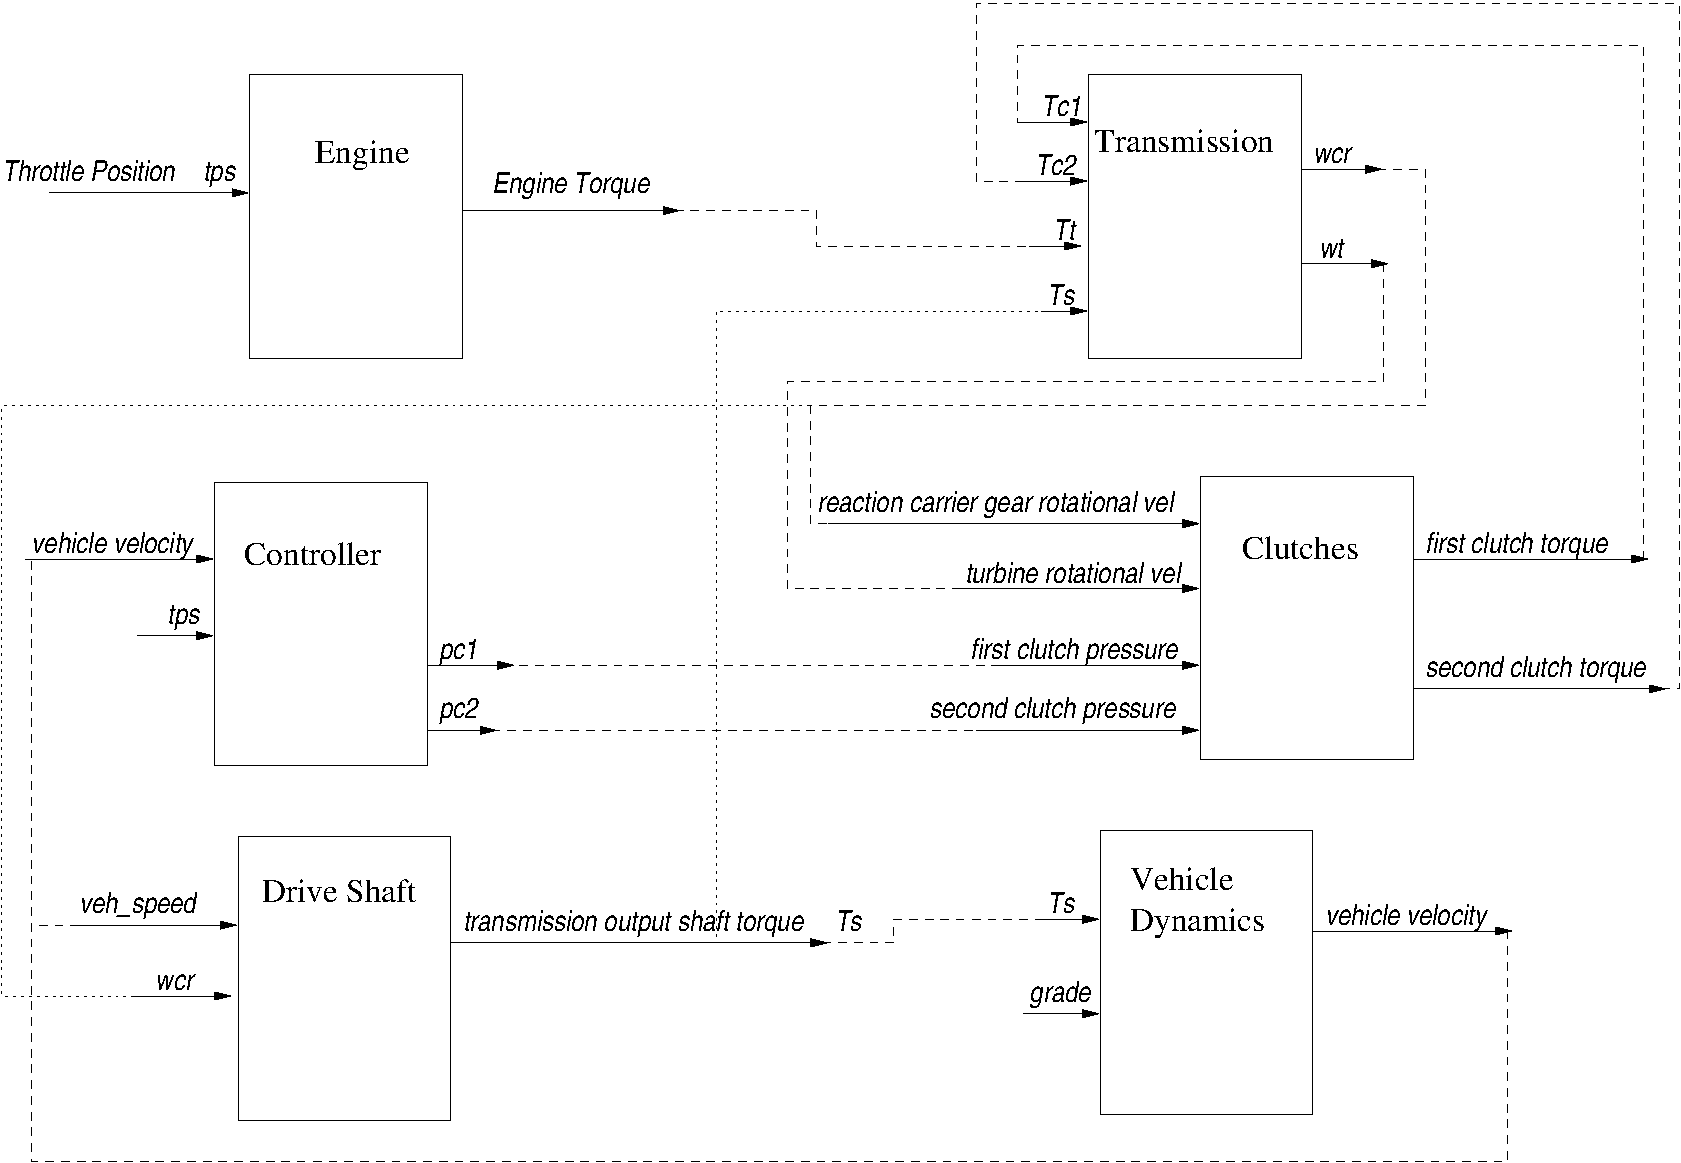
\includegraphics[angle=0,scale=0.35]{powertrain}
\end{center}

\end{slide}
% -------------------------------------------------------
\begin{slide}
\subheading{Hybrid Verification: Motivating Example}

A desired {\cem{safety}} property:

\begin{quote}
{\cem{Verification property}}: 
For a fixed grade in $[0,0.1]$ and fixed throttle in $[0,100]$,
there is no $2-1-2$ gear change sequence
\end{quote}

\medskip
Matlab can ``{\crm{verify}}'' this property for fixed 
{\cem{throttle position}} $tps$ and road $grade$

\bigskip
HybridSAL can be used to analyze it for the {\cem{whole range}}

\end{slide}
% -------------------------------------------------------
\begin{slide}
\heading{Compositionality}

{\cem{Is HybridSAL tool compositional?}}

\begin{itemize}
\item
 HybridSAL language is {\cem{hierarchical}}
 \begin{eqnarray*}
  \mathit{{\cem{HSal Module}}} := \mbox{{\cem{Composition}} of } 
  \mathit{{\cem{HSal Modules}}}
 \end{eqnarray*}

\item
 {\crm{Two}} composition operators:
 {\crm{synchronous}} and {\crm{asynchronous}}

\item
 The {\cem{abstraction}} tools work {\cem{compositionally}}
 \begin{itemize}
 \item Feedback {\cem{not}} an issue for {\cem{relational abstraction}},
 but {\cem{dilutes}} effectiveness
 \item Feedback is an issue for {\cem{qualitative abstraction}},
 only {\cem{pure predicates}} can be exchanged
 \end{itemize}

\item
 Discrete modules remain {\cem{untouched}}

\item
 The {\cem{model checkers}} work on {\cem{flattened}} modules:
 ({\cem{not compositional}})

\end{itemize}

\end{slide}
% -------------------------------------------------------
\begin{slide}
\heading{Modeling Faults, Disturbances, and Other Modes}

{\cem{HybridSAL}} is a {\crm{expressive}} specification language

\begin{itemize}
\item
 Faulty modes are {\cem{modeled explicitly}}
 \begin{itemize}
 \item  A HybridSAL system can be {\cem{multi-modal}}
 \end{itemize}

\item Distubances/noise modeled using {\cem{symbolic parameters}}
 \begin{itemize}
 \item  Semantics of HybridSAL models is {\cem{non-deterministic}}
 \item  Symbolic parameters can be {\cem{constrained}}
 \end{itemize}
\end{itemize}

\medskip
What is {\cem{not}} possible?
\begin{itemize}
\item Stochastic/probabilistic modeling and analysis
\item Partial differential equations
\end{itemize}

\end{slide}
% -------------------------------------------------------
\begin{slide}
\heading{Scalability}

HybridSAL verification tools should be used to verify
{\cem{safety-critical aspects}} of the cyber-physical system

\begin{itemize}
\item Verify safety-critical controllers/ 
 interacting cyber-physical components using {\cem{HybridSAL}}
\item Verify safety-critical communication protocols /
 distributed aspects/ state machines using {\cem{SAL}}
\end{itemize}

When the safety-critical subsystem is still {\cem{big}},
{\cem{composition/abstraction}} approach can help with 
scalability to some extent

Validated scalability {\cem{limits}}:
\begin{itemize}
\item ~25 variables for systems with linear hybrid systems
\item About 5-6 variables for systems with nonlinear hybrid systems
\item ~100 state variables for discrete state transition systems
\end{itemize}

%Approach Validated?
\end{slide}
% -------------------------------------------------------
\begin{slide}
\heading{IP and Licensing Status}

\begin{itemize}
% \item 
 % {\cem{HybridSAL parsers}}: GNU General Public License
\item
 {\cem{HybridSAL qualitative abstractor}}: GNU General Public License
\item
 {\cem{HybridSAL relational abstractor}}: META/MIT License
\item
 {\cem{SAL model checkers}}:  GNU General Public License
\item
 {\cem{Yices}}: Its own ``click-through'' license
\end{itemize}

All tools, except {\cem{Yices}}, are open source.
Free for academic/non-commercial use.

\begin{itemize}
\item HybridSAL algorithms are patented
\item HybridSAL algorithms are also published in conferences/journals
\item Algorithms in Yices are patented
\end{itemize}
% Current and intended; check SAL GNU GPL

\end{slide}
% -------------------------------------------------------
\begin{slide}
\heading{Formal Verification Tool Chain}

\hspace*{-2em}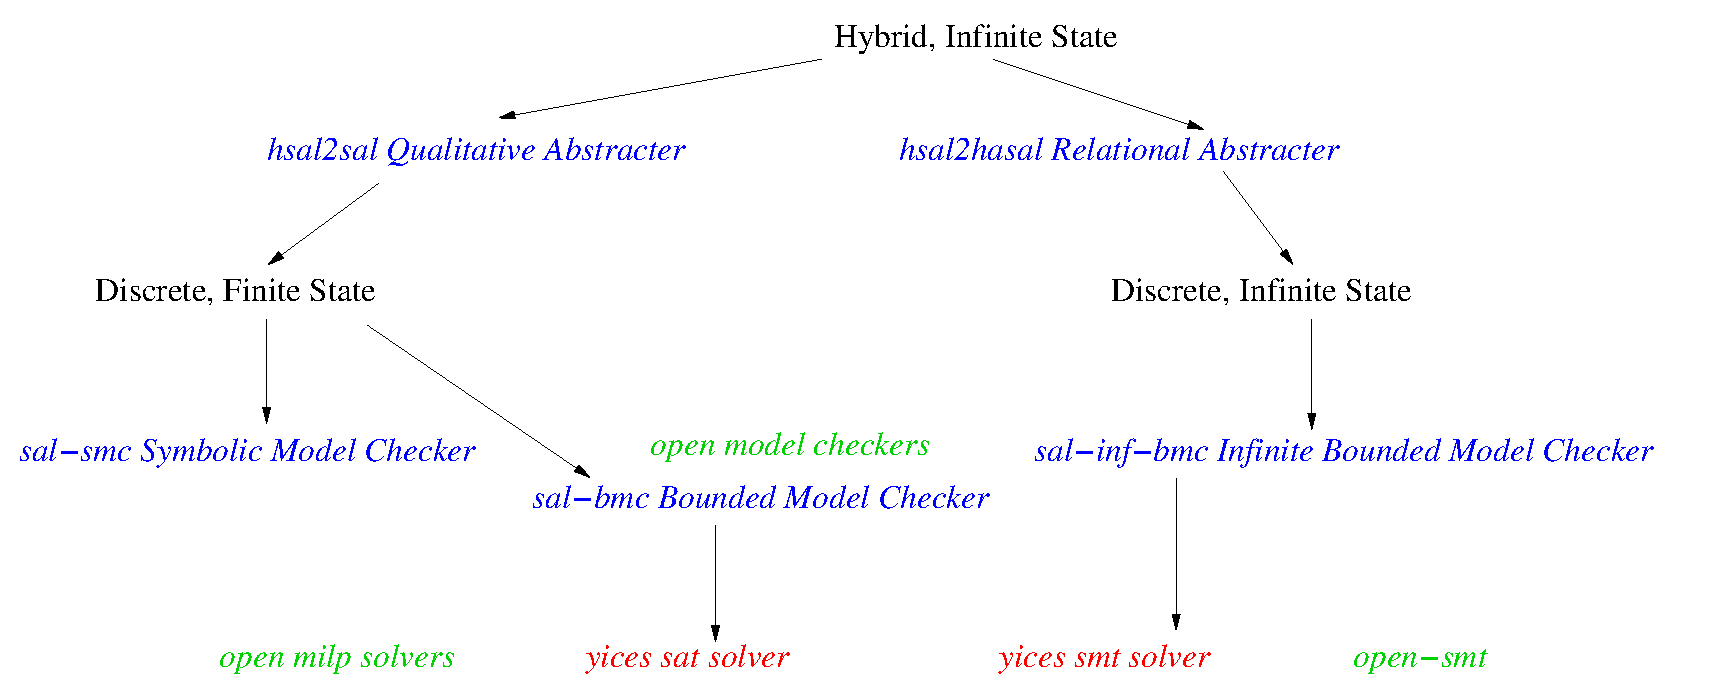
\includegraphics[angle=0,scale=0.48]{sal-tools}

\end{slide}
% -------------------------------------------------------
\begin{slide}
\heading{Platforms Supported}

HybridSAL was developed and tested on Linux

\begin{itemize}
\item
 {\cem{HybridSAL parsers}} written in antlr (needs a {\cem{java}} installation)
\item
 {\cem{HybridSAL qualitative abstractor}} written in {\cem{Lisp}}
 (developed and tested on {\crm{Allegro Lisp}})
\item
 {\cem{HybridSAL relational abstractor}} written in {\cem{Python}}
 (developed and tested on {\crm{Python 2.6 with numpy/scipy packages}})
 \\
 Also runs on {\cem{Windows platform}}
\item
 {\cem{SAL model checkers}} written in {\cem{C/C++}, {\cem{scheme}}}
 (tested on {\crm{Linux/Mac}})
\end{itemize}

%Current and intended; check website of SAL for more information/
\end{slide}
% -------------------------------------------------------
% AVM PI META notes:
% 1-page wrteup high-level summary of the tar/zip file... public release process
% MetaX : one academic tool chain (MIT licence) Vanderbilt
% One for mass market audience (paid) -- Parc CyDesign incubation
% Dassault continuig becos started late
% Verif workshop META-X focus
% IFAB - 
% Tue Nov 29 Dr Dougan at DMC keynote (defence manufacturing conf)
% -------------------------------------------------------
\end{document}
% Need slide on  Qualitative HSAL, parts,  input restrictions
% backup slide on approach

